\section{Итеративни алгоритми}

Изложените по-долу суми, може да се ползват без доказателство на контролни и домашни:

\begin{center}
	$\begin{array}{lll}
		\sum\limits_{i=1}^n1=n=\Theta(n)\qquad & \sum\limits_{i=1}^n\Theta(1)=\Theta(n)\qquad & \sum\limits_{i=c}^n=n-c+1=\Theta(n) \vspace{0.2cm}\\
		
		\sum\limits_{i=c}^n\Theta(1)=\Theta(n)\qquad & \sum\limits_{i=1}^ni=\frac{n(n+1)}2=\Theta(n^2)\qquad & \sum\limits_{i=1}^n\Theta(i)=\Theta(n^2) \vspace{0.2cm}\\
		
		\sum\limits_{\mathclap{i=1}}^ni^2=\frac{n(n+1)(2n+1)}6=\Theta(n^3)\qquad & \sum\limits_{i=1}^n\Theta(i^2)=\Theta(n^3)\qquad & \sum\limits_{\mathclap{\substack{i=1\\i=i+k}}}^n1=\lfloor\frac nk\rfloor=\Theta(n)\\
		
		\sum\limits_{\mathclap{\substack{i=1\\i=i+k}}}^n\Theta(1)=\Theta(n)\qquad & \sum\limits_{i=1}^n\frac1i=\Theta(ln(n))\qquad & \sum\limits_{i=1}^n\Theta(\frac1i)=\Theta(ln(n))\qquad
	\end{array}$
\end{center}

\begin{remark*}
	Употребата на тета-нотацията вляво на $=$ се нарича $\textbf{\emph{анонимна функция}}$
\end{remark*}

\subsection{Интегрален критерий}

В настоящия курс ще разглеждаме само частен случай на интегралния критерий, който ще ни бъде достатъчен. Това е един от най-силните инструменти, с които разполагаме, за да намираме асимптотиката на дадена сума.

%\begin{boxtheorem}[label=th-integral-criterion]{Интегрален критерий (частен случай)}{}
\begin{boxtheorem}{Интегрален критерий (частен случай)}{integral-criterion}
	Нека $f$ е $\hyperref[asym-positive]{\text{асимптотично положителна функция}}$ и нека $n_0\in\mathbb{N}_0$ е свидетел за това. Нека $\big(\exists m>0\big)\big(\exists M>0\big)\big(\forall n>n_0\big)\big(mf(n)\le\min\limits_{x\in[n,n+1]}f(x)\le\max\limits_{x\in[n,n+1]}f(x)\le Mf(n)\big)$.\\
	Тогава е изпълнено: $\displaystyle\sum_{i=n_0}^nf(i)\asymp\displaystyle\int_{n_0}^nf(x)dx$.
\end{boxtheorem}

\begin{remark*}
	Приложен интегрален критерий без посочени свидетели $m,M$ и $n_0$ и/или без обосновка на трите неравенства, носи $\textbf{нула}$ точки!
\end{remark*}\leavevmode\newline

%\vspace{0.2cm}
\subsubsection{Добре разпределени функции}
Една функиця ще наричаме $\textbf{\emph{добре разпределена}}$ (между естествените и реалните числа), ако отговаря на допълнителното условие в $\thmref{th:integral-criterion}$ за съществуване на такива константи $m$ и $M$. Нека да разгледаме малко примери за да придобием интуиция кои функции са $\textbf{\emph{добре разпределени}}$:\\

\begin{example}
	$f(x)=x^2$\\\noindent
	Ще проверим, че условието
	\begin{equation}\label{eqn-well-distributed}
		mn^2\le\min\limits_{x\in[n,n+1]}f(x)\le\max\limits_{x\in[n,n+1]}f(x)\le Mn^2
	\end{equation}
	е изпълнено за $m=1,M=4$ и произволно $n\ge n_0=1$:
	\begin{equation*}
		1n^2\le n^2\le (n+1)^2\le4n^2
	\end{equation*}
 	Първите две неравенства очевидно са верни. Остава да проверим:
 	\begin{equation*}
 		(n+1)^2\le4n^2
 	\end{equation*}
 	След като разкрием скобите получаваме:
 	\begin{equation*}
 		n^2+2n+1\le4n^2
 	\end{equation*}
 	или още
 	\begin{equation*}
 		3n^2-2n-1\ge0
 	\end{equation*}
 	Сега намираме корените $x_1=-\frac13,x_2=1$ и виждаме, че $3n^2-2n-1\ge0$ за $n\ge1$, което искахме да докажем.\\\\
 	\noindent
 	Разбира се, не е задължително да има единствени такива $m,M,n_0$. Даже напротив - ако има едно решение, то има безкрай много решения. Да разгледаме друго решение. Ще се убедим, че е изпълнено за $m=\frac13,M=1.005$ и произволно $n\ge n_0=41$:
 	\begin{equation*}
 		\frac13n^2\le n^2\le (n+1)^2\le1.005n^2
 	\end{equation*}
 	Отново първите две неравенства очевидно са верни. Остава да проверим:
 	\begin{equation*}
 		(n+1)^2\le1.005n^2
 	\end{equation*}
 	или още
 	\begin{equation*}
 		0.05n^2-2n-1\ge0
 	\end{equation*}
 	Сега намираме корените $x_1=20-2\sqrt{105}\approx-0.4939,x_2=20+2\sqrt{105}\approx40.4939$ и виждаме, че $0.05n^2-2n-1\ge0$ за $n\ge n_0=41>x_2\approx40.4939$.\\\\
 	\noindent
 	В случая кое да е $m\in(0,1]$ и кое да е $M\in(1,+\infty)$ ни вършат работа, като в зависимост от избора ни на $M$, трябва да изберем подходящо $n_0$.
\end{example}\leavevmode\newline

\begin{example}\label{exm-3-1}
	$f(x)=x^{\alpha}$\\\noindent
	В зависимост от $\alpha$ ще проверим, че условието $\ref{eqn-well-distributed}$ е изпълнено за
	\begin{mycase}
		\item $(\alpha\ge0)\ m=1,M=2^{\alpha},n_0=1$\\
		Тоест трябва да се убедим, че следните неравенства са вярни:
		\begin{equation*}
			1n^{\alpha}\le n^{\alpha}\le (n+1)^{\alpha}\le2^{\alpha}n^{\alpha}
		\end{equation*}
		Отново първите две са очевидни. Остава да се убедим само в последното неравенство:
		\begin{equation*}
			(n+1)^{\alpha}\le(2n)^{\alpha}
		\end{equation*}
		Тъй като $n_0>0$ и работим с $n\ge n_0$, то $2n>0$ и можем да разделим на него (т.е. не делим на нула и не се сменя посоката на неравенството):
		\begin{equation*}
			\bigg(\frac{n+1}{2n}\bigg)^{\alpha}\le1
		\end{equation*}
		Лесно съобразяваме, че при $n\ge n_0=1$ и $\alpha\ge0$ неравенството е изпълнено:
		\begin{equation*}
			\bigg(\underbrace{\frac{n+1}{2n}}_{\le1}\bigg)^{\alpha}\le1
		\end{equation*}
		
		\item $(\alpha<0)\ m=2^{\alpha},M=1,n_0=1$\\
		Тоест трябва да се убедим, че следните неравенства са вярни:
		\begin{equation*}
			2^{\alpha}n^{\alpha}\le (n+1)^{\alpha}\le n^{\alpha}\le1n^{\alpha}
		\end{equation*}
		Ще проверим първото неравенство, другите две са очевидни:
		\begin{equation*}
			(2n)^{\alpha}\le (n+1)^{\alpha}
		\end{equation*}
		Тъй като $n_0>0$ и работим с $n\ge n_0$, то $2n>0$ и можем да разделим на него (т.е. не делим на нула и не се сменя посоката на неравенството):
		\begin{equation*}
			\bigg(\frac{n+1}{2n}\bigg)^{\alpha}\ge1
		\end{equation*}
		Лесно съобразяваме, че при $n\ge n_0=1$ и $\alpha<0$ неравенството е изпълнено:
		\begin{equation*}
			\bigg(\underbrace{\frac{n+1}{2n}}_{\le1}\bigg)^{\alpha}=\bigg(\underbrace{\frac{2n}{n+1}}_{\ge1}\bigg)^{|\alpha|}\ge1
		\end{equation*}
	\end{mycase}
\end{example}\leavevmode\newline

\begin{example}\label{exm-3-2}
	$f(x)={\alpha}^n,\ \alpha>0$\\
	В зависимост от $\alpha$ ще проверим, че условието $\ref{eqn-well-distributed}$ е изпълнено за
	\begin{mycase}
		\item $(\alpha\ge1)\ m=1,M=\alpha,n_0=1$\\
		Тоест трябва да се убедим, че следните неравенства са вярни:
		\begin{equation*}
			1{\alpha}^n\le{\alpha}^n\le{\alpha}^{n+1}\le\alpha{\alpha}^n
		\end{equation*}
		Очевидно и трите неравенства са верни.
		
		\item $(0<\alpha<1)\ m=\alpha,M=1,n_0=1$\\
		Тоест трябва да се убедим, че следните неравенства са верни:
		\begin{equation*}
			\alpha{\alpha}^n\le{\alpha}^{n+1}\le{\alpha}^n\le1{\alpha}^n
		\end{equation*}
		Очевидно и трите неравенства са верни.
	\end{mycase}
\end{example}\leavevmode\newline

\begin{example}
	$f(x)=x^x$\\
	Това е пример за функция, която $\textbf{не}$ е добре разпределена. Убедете се защо!
\end{example}\leavevmode\newline

\begin{example}
	$f(x)=x!$\\
	Това е друг пример за функция, която $\textbf{не}$ е добре разпределена. Убедете се защо!
\end{example}\leavevmode\newline


\subsubsection{Приложения}

\begin{application}\label{apl-3-1}
	$f(x)=x^{\alpha}$\\\noindent
	Очевидно функията е асимптотично положителна и в $\exmref{exm-3-1}$ доказахме, че тя е добре разпределена. Тогава може да приложим интегралния критерий и в зависимост какво $n_0$ сме избрали получаваме:
	\begin{equation*}
		\displaystyle\sum_{i=n_0}^ni^{\alpha}\asymp\displaystyle\int_{n_0}^nx^{\alpha}dx=\begin{cases}
			\Theta(n^{\alpha+1}) &,\alpha>-1\\
			\Theta(ln(n))        &,\alpha=-1\\
			\Theta(1)            &,\alpha<-1
		\end{cases}
	\end{equation*}
\end{application}\leavevmode\newline

\begin{application}
	$f(x)={\alpha}^x,\ \alpha>0$\\\noindent
	Очевидно функията е асимптотично положителна и в $\exmref{exm-3-2}$ доказахме, че тя е добре разпределена. Тогава може да приложим интегралния критерий и в зависимост какво $n_0$ сме избрали  получаваме:
	\begin{equation*}
		\displaystyle\sum_{i=n_0}^n{\alpha}^i\asymp\displaystyle\int_{n_0}^n{\alpha}^x\,dx
	\end{equation*}
	Сега разглеждаме 3 случая в зависимост от $\alpha$:
	\begin{mycase}
		\item $(\alpha>1)$\\
		\begin{equation*}
			\displaystyle\int_{n_0}^n{\alpha}^x\,dx=\frac{{\alpha}^n-{\alpha}^{n_0}}{ln(\alpha)}=\Theta({\alpha}^n)
		\end{equation*}
		
		\item $(\alpha=1)$\\
		\begin{equation*}
			\displaystyle\int_{n_0}^n\alpha\,dx=\alpha(n-n_0)=\Theta(n)
		\end{equation*}
		
		\item $(0<\alpha<1)$\\
		\begin{equation*}
			\displaystyle\int_{n_0}^n{\alpha}^x\,dx=\frac{{\alpha}^n-{\alpha}^{n_0}}{ln(\alpha)}=\Theta(1)
		\end{equation*}
		Тъй като числителя ${\alpha}^n-{\alpha}^{n_0}$ и знаменателя $ln(\alpha)$ са строго по-малки от $0$, то цялата дроб е строго положителна. Тогава $\lim\limits_{n\to\infty}\frac{{\alpha}^n-{\alpha}^{n_0}}{ln(\alpha)}=\frac{{-\alpha}^{n_0}}{ln(\alpha)}>0$ е просто константа, откъдето имаме асимптотика $\Theta(1)$.
		
	\end{mycase}
	Тоест получихме:
	\begin{equation*}
		\displaystyle\sum_{i=n_0}^n{\alpha}^i=\begin{cases}
			\Theta({\alpha}^n) &,\alpha>1\\
			\Theta(n)          &,\alpha=1\\
			\Theta(1)          &,0<\alpha<1
		\end{cases}
	\end{equation*}
\end{application}\leavevmode\newline

\begin{application}
	Каква е асимптотиката на:

	\begin{eqnarray*}
		\text{(а) }\sum\limits_{i=1}^n\frac1i\qquad\qquad\qquad\qquad\qquad & \text{(б) }\displaystyle\sum_{i=1}^n\frac1{\sqrt{i}}\qquad\qquad\qquad\qquad\qquad & \text{(в) }\sum\limits_{i=1}^n\frac1{i^2}
	\end{eqnarray*}
\end{application}
\begin{solution}
	Това е частен случай на $\aplref{apl-3-1}$. Тоест имаме:
	\begin{eqnarray*}
		\text{(а) }\sum\limits_{i=1}^n\frac1i=\Theta(ln(n))\qquad\qquad\qquad & \text{(б) }\displaystyle\sum_{i=1}^n\frac1{\sqrt{i}}=\Theta(\sqrt{n})\qquad\qquad\qquad & \text{(в) }\sum\limits_{i=1}^n\frac1{i^2}=\Theta(1)
	\end{eqnarray*}
\end{solution}\leavevmode\newline

\begin{application}
	Каква е асимптотиката на $\sum\limits_{i=1}^nln(i)$?
\end{application}
\begin{solution}
	Очевидно е, че функцията $f(x)=ln(x)$ е асимптотично положителна. Остана да покажем, че тя е добре разпределена. Тоест трябва да намерим такива $m,M>0$ и $n_0\in\mathbb{N}_0$, че да е вярно неравенство $\ref{eqn-well-distributed}$. Ще покажем, че $m=1,M=2,n_0=2$ са свидели:
	\begin{equation*}
		1ln(n)\le ln(n)\le ln(n+1)\le 2ln(n)
	\end{equation*}
	Очевидно първите две неравенства са изпълнени. Остава да проверим третото:
	\begin{equation*}
		ln(n+1)\le 2ln(n)=ln(n^2)
	\end{equation*}
	Нека се убедим първо, че следното неравенство е изпълнено за $n\ge n_0=2$:
	\begin{equation*}
		n+1\le n^2
	\end{equation*}
	или още
	\begin{equation*}
		n^2-n-1\ge0
	\end{equation*}
	Сега намираме корените $x_1=\frac{1-\sqrt5}{2}\approx-0.618,x_2=\frac{1+\sqrt5}{2}\approx1.618$ и виждаме, че $n^2-n-1\ge0$ за $n\ge n_0=2>x_2\approx1.618$.
	Знаем, че логаритмуването на асимптотично положителни и неограничени отгоре функции запазва посоката на неравенството, откъдето получаваме:
	\begin{equation*}
		ln(n+1)\le ln(n^2)=2ln(n)
	\end{equation*}
	Сега вече може да приложим интегралния критерий, откъдето получаваме:
	\begin{eqnarray*}
		\displaystyle\sum_{i=2}^nln(i)\asymp\displaystyle\int_2^nln(x)\,dx & = & ln(x)x\Big|^n_2-\displaystyle\int_2^nx\,d(ln(x))=nln(n)-2ln(2)-\displaystyle\int_2^n\frac xx\,dx= \\
		& = & nln(n)-2ln(2)-x\Big|^n_2=nln(n)-n+2-2ln(2)=\Theta(n.ln(n))
	\end{eqnarray*}
	Забележете, че в оригиналната задача, сумата започваше от 1, а интегралния критерий ни даде асимптотика от 2 нагоре. Това обаче не е проблем, тъй като сме изпуснали $n_0-1$ на брой крайни събираеми (което е константа). Тоест имаме:
	\begin{equation*}
		\displaystyle\sum_{i=1}^nln(i)=const+\displaystyle\sum_{i=2}^nln(i)=const+\Theta(n.ln(n))=\Theta(n.ln(n))
	\end{equation*}
	В случая даже изпуснатото събираемо е $ln(1)=0$, но в общия случай това не е така.
\end{solution}\leavevmode\newline

\begin{application}
	Каква е асимптотиката на $\sum\limits_{i=1}^n\frac{ln(i)}{i}$?
\end{application}
\begin{solution}
	За упражнение докажете (използвайки интегралния критерий), че:
	\begin{equation*}
		\sum\limits_{i=1}^n\frac{ln(i)}{i}\asymp\Theta(ln^2(n))
	\end{equation*}
\end{solution}\leavevmode\newline


\subsection{Задачи}

Основната идея е да заместим всяка атомарна операция с константа (или за по-лесно единица - не се отразява на асимптотиката), а циклите с математическа сума. Нека разгледаме няколко примерни задачи:\\

\begin{problem}
	Даден е следният алгоритъм:
	\begin{pseudocode}
		\SetKwData{di}{i}
		\SetKwData{dn}{n}
		
		$Func(\dn)://\,\dn\in\mathbb{N}^+$
		\Mybegin
		{
			print 'a'\;
			\Myfor{$\di\leftarrow1$ \KwTo $\dn$}{print 'b'\;}
			fastprint 'c'\;
			print 'd'\;
		}
	\end{pseudocode}
	Каква е сложността му по време (спрямо $n$)?
\end{problem}
\begin{solution}
	Сложността му по време е $c_{print}+\sum\limits_{i=1}^n(c_{print}+c_{checkend}+c_{increment})+c_{fastprint}+c_{print}=2c_{print}+n(c_{print}+c_{checkend}+c_{increment})+c_{fastprint}=\Theta(n)$.
\end{solution}

\begin{remark*}
	За чистота се разбираме да пишем $1$ вместо $c_{name}$ за всички атомарни операции.
\end{remark*}\leavevmode\newline

\begin{problem}
	Даден е следният алгоритъм:
	\begin{pseudocode}
		\SetKwData{di}{i}
		\SetKwData{dj}{j}
		\SetKwData{dn}{n}
		
		$Func(\dn)://\,\dn\in\mathbb{N}^+$
		\Mybegin
		{
			\Myfor{$\di\leftarrow1$ \KwTo $\dn$}
			{
				\Myfor{$\dj\leftarrow1$ \KwTo $\dn$}{print 'a'\;}
			}
		}
	\end{pseudocode}
	Каква е сложността му по време (спрямо $n$)?
\end{problem}
\begin{solution}
	Сложността му по време е $\sum\limits_{i=1}^n\sum\limits_{j=1}^n1=\sum\limits_{i=1}^n n=n\sum\limits_{i=1}^n 1=n\,n=\Theta(n^2)$.
\end{solution}\leavevmode\newline

\begin{problem}
	Даден е следният алгоритъм:
	\begin{pseudocode}
		\SetKwData{di}{i}
		\SetKwData{dj}{j}
		\SetKwData{dn}{n}
		
		$Func(\dn)://\,\dn\in\mathbb{N}^+$
		\Mybegin
		{
			\Myfor{$\di\leftarrow1$ \KwTo $\dn$}
			{
				\Myfor{$\dj\leftarrow1$ \KwTo $\di$}{print 'a'\;}
			}
		}
	\end{pseudocode}
	Каква е сложността му по време (спрямо $n$)?
\end{problem}
\begin{solution}
	Сложността му по време е $\sum\limits_{i=1}^n\sum\limits_{j=1}^i1=\sum\limits_{i=1}^n i=\frac{(n+1)n}{2}=\Theta(n^2)$.
\end{solution}\leavevmode\newline

\begin{problem}
	Даден е следният алгоритъм:
	\begin{pseudocode}
		\SetKwData{di}{i}
		\SetKwData{dj}{j}
		\SetKwData{dn}{n}
		
		$Func(\dn)://\,\dn\in\mathbb{N}^+$
		\Mybegin
		{
			\Myfor{$\di\leftarrow1$ \KwTo $\dn$}
			{
				\Myfor(\Withstep $\di$){$\dj\leftarrow1$ \KwTo $\dn$}{print 'a'\;}
			}
		}
	\end{pseudocode}
	Каква е сложността му по време (спрямо $n$)?
\end{problem}
\begin{solution}
	Сложността му по време$\,$е$\,\sum\limits_{i=1}^n\sum\limits_{\substack{j=1\\j=j+i}}^n1=\sum\limits_{i=1}^n\lfloor\frac ni\rfloor\asymp\sum\limits_{i=1}^n\frac ni=n\sum\limits_{i=1}^n\frac1i\asymp nln(n)=\Theta(n\,ln(n))$.
\end{solution}\leavevmode\newline

\begin{boxremark}{Сложност спрямо големината на входа}{}
	Забележете, че големината на входа на горните четири задачи (а и на долната) е все $log(n)$. Тоест сложността по време (спрямо големината на входа $m=log(n)$) на горните четири задачи е съответно $\Theta(2^m),\Theta((2^m)^2)=\Theta(4^m),\Theta(4^m)$ и $\Theta(2^mlog(2^m))=\Theta(m2^m)$.
\end{boxremark}\leavevmode\newline

\begin{problem}
	Даден е следният алгоритъм:
	\begin{pseudocode}
		\SetKwData{di}{i}
		\SetKwData{dj}{j}
		\SetKwData{dk}{k}
		\SetKwData{dn}{n}
		
		$Func(\dn)://\,\dn\in\mathbb{N}^+$
		\Mybegin
		{
			\Myfor{$\di\leftarrow1$ \KwTo $\dn$}
			{
				\Myfor{$\dj\leftarrow i$ \KwTo $2^i$}
				{
					\If{$\dj<\dn$}
					{
						\Myfor(\Withstep $\di$){$\dk\leftarrow1$ \KwTo $\dn$}{print 'a'\;}
					}
					print 'b'\;
				}
				
				
				
				%\Myfor(\Withstep $\di$){$\dj\leftarrow1$ \KwTo $\dn$}{print 'a'\;}
			}
		}
	\end{pseudocode}
	Каква е сложността му по време (спрямо $n$, а спрямо големината на входа $m=log(n)$)?
\end{problem}
\begin{solution}
	Сложността му по време е:
	\begin{equation}\label{eqn-3-1}
		\underbrace{\sum\limits_{i=1}^{n}\sum\limits_{j=i}^{2^i}1}_{\text{print 'b'}}+\underbrace{\sum\limits_{i=1}^{\lfloor log(n)\rfloor}\sum\limits_{j=i}^{2^i}\sum\limits_{\substack{k=1\\k=k+i}}^n1}_{\text{print 'a' }(i\le\lfloor log(n)\rfloor)}+\underbrace{\sum\limits_{i=\lfloor log(n)\rfloor+1}^n\sum\limits_{j=i}^n\sum\limits_{\substack{k=1\\k=k+i}}^n1}_{\text{print 'a' }(i>\lfloor log(n)\rfloor)}
	\end{equation}
	Нека да разгледаме трите суми поотделно. Да започнем с първата:
	\begin{equation*}
		\sum\limits_{i=1}^n\sum\limits_{j=i}^{2^i}1=\sum\limits_{i=1}^n\Big(2^i-i+1\Big)=\sum\limits_{i=1}^n2^i-\sum\limits_{i=1}^ni+\sum\limits_{i=1}^n1\asymp2^n-n^2+n=\Theta(2^n)
	\end{equation*}
	Сега да разгледаме втората (като премахнем закръглянето - не променя асимптотиката):
	\begin{eqnarray*}
		\sum\limits_{i=1}^{log(n)}\sum\limits_{j=i}^{2^i}\sum\limits_{\substack{k=1\\k=k+i}}^n1 &\asymp& 
		\sum\limits_{i=1}^{log(n)}\sum\limits_{j=i}^{2^i}\frac ni =
		n\sum\limits_{i=1}^{log(n)}\bigg(\frac1i\sum\limits_{j=i}^{2^i}1\bigg) =
		n\sum\limits_{i=1}^{log(n)}\bigg(\frac1i\Big(2^i-i+1\Big)\bigg) =\\
		&=&
		n\Bigg(\sum\limits_{i=1}^{log(n)}\frac{2^i}i-\sum\limits_{i=1}^{log(n)}\frac ii+\sum\limits_{i=1}^{log(n)}\frac1i\Bigg) \le
		n\Bigg(\sum\limits_{i=1}^{log(n)}2^i-\sum\limits_{i=1}^{log(n)}1+\sum\limits_{i=1}^{log(n)}\frac1i\Bigg) \asymp \\
		&\asymp&
		n\Big(2^{log(n)}-log(n)+ln(log(n))\Big) \asymp n\Big(n-log(n)+log^{(2)}(n)\Big) \asymp n^2
	\end{eqnarray*}
	В крайна сметка за втората сума получихме:
	\begin{equation*}
		\sum\limits_{i=1}^{log(n)}\sum\limits_{j=i}^{2^i}\sum\limits_{\substack{k=1\\k=k+i}}^n1=O(n^2)
	\end{equation*}
	Обърнете внимание, че е $O(n^2)$, а не $\Theta(n^2)$ - това е заради употребата на $\le$. Разбира се може в действителност да е $\Theta(n^2)$, но $O(n^2)$ ни е достатъчно (след малко ще видим защо) да определим сложността по време на $\ref{eqn-3-1}$. Остана да разгледаме третата сума (отново махаме закръглянето и константата +1 - не променят асимптотиката):
	\begin{eqnarray*}
		\sum\limits_{i=log(n)}^n\sum\limits_{j=i}^n\sum\limits_{\substack{k=1\\k=k+i}}^n1 &\asymp&
		\sum\limits_{i=log(n)}^n\sum\limits_{j=i}^n\frac ni =
		n\sum\limits_{i=log(n)}^n\frac1i\sum\limits_{j=i}^n1 =
		n\sum\limits_{i=log(n)}^n\bigg(\frac1i\Big(n-i+1\Big)\bigg) = \\
		&=&
		n\Bigg(n\sum\limits_{i=log(n)}^n\frac1i-\sum\limits_{i=log(n)}^n\frac{log(n)}i+\sum\limits_{i=log(n)}^n\frac1i\Bigg) = 
		\dots =
		\Theta(n^2log(n))		
	\end{eqnarray*}
	Тоест сложността по време на функцията е $\Theta(2^n)+O(n^2)+\Theta(n^2log(n))=\Theta(2^n)=\Theta(2^{2^m})$.
\end{solution}\newpage


\section{Рекурсивни алгоритми}\label{sec-rec-alg}

Сложността на рекурсивни алгоритми ще определяме посредством рекурентни уравнения. По тази причина рекурентните уравнения, които ще разглеждаме ще са със строго намаляващ аргумент, всички нехомогенни събираеми отдясно на $=$ ще се срещат с положителен знак и всички основи на експоненти в нехомогенната част ще бъдат положителни. Също така да обърнем внимание, че за всяко фиксирано $n_0\in\mathbb{N}_0$ е изпълнено $\big(\forall n\le n_0\big)\big(T(n)=\Theta(1)\big)$, където $T(n)$ е рекурентно уравнение. Може да си мислим за това $n_0$ като базата на рекурсивния алгоритъм. За удобство ще нагласяме $n_0$ да е някое малко число - например $0,1,2$ - в зависимост от конкретната задача. Съставянето на рекурентно уравнение за сложността на рекурсивен алгоритъм е тривиално в повечето случаи. Поради тази причина ще се съсредоточим върху методи за намиране на асимптотиката на рекурентни уравнения.\\

\subsection{Характеристично уравнение}

Започваме с метод, който ви е добре познат от ДСТР. За разлика от ДСТР, тук не ни интересува точното решение, а само асимптотиката.

\begin{problem}\label{prob-3-1}
	Каква е асимптотиката на $T(n)=4T(n-2)+n2^n+4\cdot3^n$?
\end{problem}
\begin{solution}
	\noindent
	\begin{itemize}
		\item (Хомогенна част)\\
		$x^2=4\ \mapsto\ x_{1,2}=\pm2\ \mapsto\ \{2,-2\}_M$
		
		\item (Нехомогенна част)
		\begin{itemize}
			\item $n2^n\ \mapsto\ \{2,2\}_M$
			\item $4\cdot3^n\ \mapsto\ \{3\}_M$
		\end{itemize}
	\end{itemize}
	Като обединим всички мултимножества получаваме: $\{-2,2,2,2,3\}_M$. Оттук получаваме, че $T(n)=c_1(-2)^n+c_22^n+c_3n2^n+c_4n^22^n+c_53^n=\Theta(3^n)$.
\end{solution}

\begin{remark*}
	Забележете, че поради естеството на рекурентните уравнения (строго намаляващ аргумент, положителен знак отдясно на $=$ и положителна основа на експонентата в нехомогенната част), то ни е гарантирано, че най-голямото (по модул) число в крайното мултимножество ще е положително и при това ще се среща със строго положителна константа в явния запис на рекурентното уравнение. Поради тази причина в $\probref{prob-3-1}$ сме сигурни, че $c_5>0$ (и че $\max\{|-2|,|2|,|2|,|2|,|3|\}=3\in\{-2,2,2,2,3\}$).
\end{remark*}\leavevmode\newline

\begin{problem}
	Каква е асимптотиката на $T(n)=2T(n-1)+T(n-2)$?
\end{problem}
\begin{solution}
	Тук имаме само хомогенна част: $x^2=2x+1\ \mapsto\ x_{1,2}=1\pm\sqrt2\ \mapsto\ \{1+\sqrt2,1-\sqrt2\}_M$. Оттук получаваме $T(n)=c_1(1+\sqrt2)^n+c_2(1-\sqrt2)^n=\Theta((1+\sqrt2)^n)$.
\end{solution}\leavevmode\newline

\begin{problem}\label{prob-rec-eq-full-history}
	Каква е асимптотиката на $T(n)=T(n-2)+T(n-4)+\dots+\underbrace{T(n\%2)}_{T(0)\text{ или }T(1)}$?
\end{problem}
\begin{solution}
	Това характеристично уравнение се решава със следния трик:
	$T(n)-T(n-2)=\underbrace{T(n-2)+T(n-4)+\dots+T(n\%2)}_{T(n)}-(\underbrace{T(n-4)+T(n-6)+\dots+T(n\%2)}_{T(n-2)})=T(n-2)$. Тоест получихме, че $T(n)-T(n-2)=T(n-2)$ или още $T(n)=2T(n-2)$. Решаваме характеристичното уравнение $x^2=2$ и получаваме $x_{1,2}=\pm\sqrt2\ \mapsto\ \{\sqrt2,-\sqrt2\}_M$. Оттук имаме $T(n)=c_1(\sqrt2)^n+c_2(-\sqrt2)^n=\Theta((\sqrt2)^n)$.
\end{solution}\leavevmode\newline


\subsection{Развиване}

Метода за намиране асимптотика на рекурентно уравнение чрез развиване е най-мощният, който ще разгледаме в текущия курс, но и най-хамалският. Изисква сравнително много писане и известна доза $\emph{умен съм бил сетил съм се}$ (зависи от задачата). Самия метод не е формален. Формализацията изисква доказателство чрез индукция, което е трудната част. Идеята е много проста - развиваме докажо не заподозреем сложността и след това доказваме формално.

\begin{problem}
	Каква е асимптотиката на $T(n)=T(n-1)+n$?
\end{problem}
\begin{solution}
	Тази задача може да се реши чрез характеристично уравнение, но сега ще го докажем чрез развиване и индукция.
	\begin{eqnarray*}
		T(n)
		&=& T(n-1)+n=T(n-2)+(n-1)+n=\\
		&=& T(n-3)+(n-2)+(n-1)+n=\dots=\\
		&=& T(0)+1+2+\dots+(n-1)+n=T(0)+\Theta(n^2)=\Theta(n^2)
	\end{eqnarray*}
	\begin{boxremark*}{}{}
		Дотук $\textbf{НЕ}$ сме доказали нищо! Само сме заподозрели отговора! Проблема е в това, че употребата на "$\dots$"\ е изцяло неформална.. може да сме сбъркали нещо на ум!
	\end{boxremark*}
	\noindent
	Нека $n_{st}\in\mathbb{N}_0$ е достатъчно голямо\footnote{Надолу в доказателството ще въведем $n_0$ и ще изискваме $n_0<n_{st}$.}.
	\begin{itemize}
		\item $T(n)=O(n^2)$
		
		По $\hyperref[bdef-asymp-classes]{\text{дефиниция}}$ имаме $O(n^2)=\{f\in\mathscr{F}^+|\big(\exists c>0\big)\big(\exists n_0\in\mathbb{N}_0\big)\big(\forall n\ge n_0\big)\big(0\le f(n)\le cn^2\big)\}$. Тоест търсим константи $c>0$ и $n_0\in\mathbb{N}_0$ такива, че $\big(\forall n\ge n_0\big)\big(0\le T(n)\le cn^2\big)$. Както се разбрахме в началото на $\ref{sec-rec-alg}$, сложността на рекурсивните алгоритмите, които ще разглеждаме в текущия курс, изпълняват условието $T(n)\ge0$. Тоест търсим константи $c>0$ и $n_0\in\mathbb{N}_0$ такива, че $\big(\forall n\ge n_0\big)\big(T(n)\le cn^2\big)$.
		
		Нека $b=\max\Bigl\{\frac{T(1)}{1^2},\frac{T(2)}{2^2},\frac{T(3)}{3^2},\dots,\frac{T(n_{\text{st}}-1)}{({n_{\text{st}}-1)^2}},1$\footnote{Надолу ще установим, защо добавяме тази единица.}$\Bigr\}$. (виж $\remref{rem:rec-base}$)
		
		Ще докажем с индукция по $n$, че за $c=b$ и някое $n_0$ (което ще установим по-надолу) е изпълнено $\big(\forall n\ge n_0\big)\big(T(n)\le cn^2\big)$.\\\\
		
		\begin{base}
			Нека $k\in\{1,2,\dots,n_{st}-1\}$. Ще докажем, че $T(k)\le bk^2$.
			
			От дефиницията на $b=\max\Bigl\{\frac{T(1)}{1^2},\frac{T(2)}{2^2},\frac{T(3)}{3^2},\dots,\frac{T(n_{\text{st}}-1)}{({n_{\text{st}}-1)^2}},1\Bigr\}$ знаем, че $b\ge \frac{T(k)}{k^2}$ откъдето $bk^2\ge T(k)$ или още $T(k)\le bk^2$.
		\end{base}
	
		\begin{indhypothesis}
			Нека допуснем, че е изпълнено $\big(\forall m<n\big)\big(T(m)\le bm^2\big)$.
		\end{indhypothesis}
	
		\begin{indstep}
			Ще докажем, че е изпълнено за $n$, тоест че $T(n)\le bn^2$.
			
			\begin{equation*}
				T(n)\overset{\text{def}}{=}T(n-1)+n\overset{\text{ИХ}}{\le}b(n-1)^2+n=bn^2-2bn+b+n\overset{?}{\le}bn^2
			\end{equation*}
			\begin{equation*}
				bn^2-2bn+b+n\overset{?}{\le}bn^2
			\end{equation*}
			\begin{equation*}
				n(1-2b)+b\overset{?}{\le}0
			\end{equation*}
		
			Може да забележим, че при $1-2b\le-b$ горното неравенство ще е изпълнено за всяко $n\ge1$. Оттук си избираме $n_0=1$.
			
			Остана да видим кога е изпълнено $1-2b\le-b$. Очевидно е изпълнено когато $b\ge1$. Това сме си го подсигурили от дефиницията на $b=\max\{\dots,1\}\Rightarrow b\ge1$.
		\end{indstep}
		
		Тоест доказахме, че за $c=b\land n_0=1$ е изпълнено $\big(\forall n\ge n_0\big)\big(0\le T(n)\le cn^2\big)$. Казано с други думи $T(n)=O(n^2)$.
		
		\vspace{0.35cm}
		\item $T(n)=\Omega(n^2)$
		
		По $\hyperref[bdef-asymp-classes]{\text{дефиниция}}$ имаме $\Omega(n^2)=\{f\in\mathscr{F}^+|\big(\exists c>0\big)\big(\exists n_0\in\mathbb{N}_0\big)\big(\forall n\ge n_0\big)\big(0\le cn^2\le f(n)\big)\}$. Тоест търсим константи $c>0$ и $n_0\in\mathbb{N}_0$ такива, че $\big(\forall n\ge n_0\big)\big(cn^2\le T(n)\big)$.
		
		Нека $b=\min\Bigl\{\frac{T(1)}{1^2},\frac{T(2)}{2^2},\frac{T(3)}{3^2},\dots,\frac{T(n_{\text{st}}-1)}{({n_{\text{st}}-1)^2}},\frac12\Bigr\}$. (виж $\remref{rem:rec-base}$)
		
		Ще докажем с индукция по $n$, че за $c=b$ и някое $n_0$ (което ще установим по-надолу) е изпълнено $\big(\forall n\ge n_0\big)\big(cn^2\le T(n)\big)$.
		
		\begin{base}
			Нека $k\in\{1,2,\dots,n_{st}-1\}$. Ще докажем, че $bk^2\le T(k)$.
			
			От дефиницията на $b=\min\Bigl\{\frac{T(1)}{1^2},\frac{T(2)}{2^2},\frac{T(3)}{3^2},\dots,\frac{T(n_{\text{st}}-1)}{({n_{\text{st}}-1)^2}},\frac12\Bigr\}$ знаем, че $b\le \frac{T(k)}{k^2}$ откъдето $bk^2\le T(k)$.
		\end{base}
		
		\begin{indhypothesis}
			Нека допуснем, че е изпълнено $\big(\forall m<n\big)\big(bm^2\le T(m)\big)$.
		\end{indhypothesis}
	
	\begin{indstep}
		Ще докажем, че е изпълнено за $n$, тоест че $bn^2\le T(n)$.
		
		\begin{equation*}
			T(n)\overset{\text{def}}{=}T(n-1)+n\overset{\text{ИХ}}{\ge}b(n-1)^2+n=bn^2-2bn+b+n\overset{?}{\ge}bn^2
		\end{equation*}
%		\begin{equation*}
%			bn^2-2bn+b+n\overset{?}{\ge}bn^2
%		\end{equation*}
		\begin{equation*}
			n(1-2b)+b\overset{?}{\ge}0
		\end{equation*}
	
		Може да забележим, че при $1-2b\ge0$ горното неравенство ще е изпълнено за всяко $n\ge0$. Оттук си избираме $n_0=1$ (ако изберем $n_0=0$ ще имаме $\frac{T(0)}{0}$).
		
		Остана да видим кога е изпълнено $1-2b\ge0$. Очевидно е изпълнено когато $b\le\frac12$.\qquad Това сме си го подсигурили от дефиницията на $b=\min\{\dots,\frac12\}\Rightarrow b\le\frac12$.
	\end{indstep}

	Тоест доказахме, че за $c=b\land n_0=1$ е изпълнено $\big(\forall n\ge n_0\big)\big(0\le cn^2\le T(n)\big)$. Казано с други думи $T(n)=\Omega(n^2)$.
		
	\end{itemize}
\end{solution}

\newpage

\begin{boxremark}{Константата $\hyperref[bdef-asymp-classes]{\color{green}c}$ при доказване с индукция}{rec-base}
	Когато доказваме, че асимптотиката на рекурентно уравнение е $\varphi(n)$ чрез индукция, то константата винаги е от вида $\max$ (за $O$) или $\min$ (за $\Omega$) на $\{\frac{T(n_0)}{\varphi(n_0)},\frac{T(n_0+1)}{\varphi(n_0+1)},\dots,\frac{T(n_{st}-1)}{\varphi(n_{st}-1)}\}$, като внимаваме за избора на $n_0$ - да не разделим на нула (примерно ако $\varphi(n)=log(n)$, то тогава $\frac{T(1)}{\varphi(1)}=\frac{T(1)}0$). Потенциално може да трябва още един елемент към множеството.
	
	Нека разгледаме няколко примерни константи:
	\begin{itemize}
		\item $T(n)=O(n^2)\mapsto\max\Bigl\{\frac{T(1)}{1^2},\frac{T(2)}{2^2},\frac{T(3)}{3^2},\dots,\frac{T(n_{\text{st}}-1)}{({n_{\text{st}}-1)^2}},\textcolor{red}?\Bigr\}$
		
		\item $T(n)=\Omega(log(n))\mapsto\min\Bigl\{\frac{T(2)}{log(2)},\frac{T(3)}{log(3)},\dots,\frac{T(n_{\text{st}}-1)}{log(n_{st}-1)},\textcolor{red}?\Bigr\}$
		
		\item $T(n)=O(2^n)\mapsto\max\Bigl\{\frac{T(0)}{2^0},\frac{T(1)}{2^1},\frac{T(2)}{2^2},\dots,\frac{T(n_{\text{st}}-1)}{2^{(n_{st}-1)}},\textcolor{red}?\Bigr\}$
		
		\item $T(n)=\Omega(n^3-4n^2+3n)\mapsto\min\Bigl\{\frac{T(4)}{4^3-4\cdot4^2+3\cdot4},\frac{T(5)}{5^3-4\cdot5^2+3\cdot5},\dots,\frac{T(n_{\text{st}}-1)}{(n_{st}-1)^3-4(n_{st}-1)^2+3(n_{st}-1)},\textcolor{red}?\Bigr\}$
	\end{itemize}
	Важно е да обърнем внимание, че при образуването на базата има разлика между $\Omega(n^3-4n^2+3n)$, $\Omega(n^3)$ и $\Omega(5n^3)$. Пример защо това е важно в $O$-посоката на $\probref{prob-ind-str}$.
\end{boxremark}\leavevmode\newline

\begin{problem}
	Каква е асимптотиката на $T(n)=T(n-1)+\frac1n$?
\end{problem}
\begin{solution}
	Нека да развием, докато не заподозреем асимптотиката.
	\begin{eqnarray*}
		T(n)
		&=& T(n-1)+\frac1n=T(n-2)+\frac1{n-1}+\frac1n=\\
		&=& T(n-3)+\frac1{n-2}+\frac1{n-1}+\frac1n=\dots=\\
		&=& T(0)+\frac11+\frac12+\dots+\frac1{n-1}+\frac1n=T(0)+\Theta(ln(n))=\Theta(log(n))
	\end{eqnarray*}
	Нека $n_{st}\in\mathbb{N}_0$ е достатъчно голямо.
	
	\begin{itemize}
		\item $T(n)=O(log(n))$
		
		По $\hyperref[bdef-asymp-classes]{\text{дефиниция}}$ $O(log(n))\!=\!\{f\in\mathscr{F}^+|\big(\exists c>0\big)\big(\exists n_0\in\mathbb{N}_0\big)\big(\forall n\ge n_0\big)\big(0\le f(n)\le c\,log(n)\big)\}$. Тоест търсим $c>0$ и $n_0\in\mathbb{N}_0$ такива, че $\big(\forall n\ge n_0\big)\big(T(n)\le c\,log(n)\big)$.
		
		Нека $b=\max\Bigl\{\frac{T(2)}{log(2)},\frac{T(3)}{log(3)},\frac{T(4)}{log(4)},\dots,\frac{T(n_{\text{st}}-1)}{log({n_{\text{st}}-1)}},1\Bigr\}$.% (виж $\remref{rem:rec-base}$)
		
		Ще докажем с индукция по $n$, че за $c=b$ и някое $n_0$ (което ще установим по-надолу) е изпълнено $\big(\forall n\ge n_0\big)\big(T(n)\le c\,log(n)\big)$.
		
		\begin{base}
			Нека $k\in\{2,3,\dots,n_{st}-1\}$. Ще докажем, че $T(k)\le b\,log(k)$.
			
			От дефиницията на $b=\max\Bigl\{\frac{T(2)}{log(2)},\frac{T(3)}{log(3)},\frac{T(4)}{log(4)},\dots,\frac{T(n_{\text{st}}-1)}{log({n_{\text{st}}-1)}},1\Bigr\}$ знаем, че $b\ge \frac{T(k)}{log(k)}$ откъдето $b\,log(k)\ge T(k)$ или още $T(k)\le b\,log(k)$.
		\end{base}
	
		\begin{indhypothesis}
			Нека допуснем, че е изпълнено $\big(\forall m<n\big)\big(T(m)\le b\,log(m)\big)$.
		\end{indhypothesis}
	
		\begin{indstep}
			Ще докажем, че е изпълнено за $n$, тоест че $T(n)\le b\,log(n)$.
			
			\begin{equation*}
				T(n)\overset{\text{def}}{=}T(n-1)+\frac1n\overset{\text{ИХ}}{\le}b\,log(n-1)+\frac1n\overset{?}{\le}b\,log(n)
			\end{equation*}
			\begin{equation*}
				b\,log(n-1)+\frac1n\overset{?}{\le}b\,log(n)
			\end{equation*}
			Тъй като $n\ge n_0\in\mathbb{N}_0$, то може да умножим по $n$ без да се обърне знака на неравенството.
			\begin{equation*}
				bn\,log(n-1)+1\overset{?}{\le}bn\,log(n)
			\end{equation*}
			\begin{equation*}
				1\overset{?}{\le}bn\,log(n)-bn\,log(n-1)
			\end{equation*}
			\begin{equation*}
				1\overset{?}{\le}bn\,log\bigg(\frac{n}{n-1}\bigg)
			\end{equation*}
			Антилогаритмуваме двете страни (със основа 2)
			\begin{equation*}
				2\overset{?}{\le}\bigg(\frac{n}{n-1}\bigg)^{bn}
			\end{equation*}
			От дефиницията на $b\!=\!\max\{\dots,1\}\Rightarrow b\ge1$. Ясно е, че $\big(\forall n\ge1\big)\big(\frac{n}{n-1}\ge1\big)$. Тоест имаме:
			\begin{equation*}
				2\overset{?}{\le}\bigg(\frac{n}{n-1}\bigg)^n\le\bigg(\frac{n}{n-1}\bigg)^{bn}
			\end{equation*}
			\begin{equation*}
				2\overset{?}{\le}\bigg(\frac{n}{n-1}\bigg)^{n-1}\le\bigg(\frac{n}{n-1}\bigg)^n
			\end{equation*}
			От анализа знаем, че $\lim\limits_{n\to\infty}\big(\frac{n}{n-1}\big)^{n-1}=e$ и че функцията $\big(\frac{n}{n-1}\big)^{n-1}$ е строго растяща. Тогава директно проверяваме, че $n_0=2$ ни върши работа% Тоест $\forall n\ge n_0\,\big(2\le\big(\frac{n}{n-1}\big)^{n-1}\big)$. 
			\begin{equation*}
				\big(\forall n\ge n_0\big)\Bigg(2\le\bigg(\frac{n}{n-1}\bigg)^{n-1}\le\bigg(\frac{n}{n-1}\bigg)^{bn}\Bigg)
			\end{equation*}
			или още
			\begin{equation*}
				\big(\forall n\ge n_0\big)\Bigg(2\le\bigg(\frac{n}{n-1}\bigg)^{bn}\Bigg)
			\end{equation*}
			Тъй като логаритмуването е монотонно растяща функция, то можем да запазим неравенството след логаритмуване на двете страни
			\begin{equation*}
				\big(\forall n\ge n_0\big)\Bigg(1\le bn\,log\bigg(\frac{n}{n-1}\bigg)\Bigg)
			\end{equation*}
			което трябваше да докажем.
		\end{indstep}
	
		\vspace{0.35cm}
		\item $T(n)=\Omega(log(n))$
		
		По $\hyperref[bdef-asymp-classes]{\text{дефиниция}}$ $\Omega(log(n))\!=\!\{f\in\mathscr{F}^+|\big(\exists c>0\big)\big(\exists n_0\in\mathbb{N}_0\big)\big(\forall n\ge n_0\big)\big(0\le c\,log(n)\big)\le f(n)\}$. Тоест търсим $c>0$ и $n_0\in\mathbb{N}_0$ такива, че $\big(\forall n\ge n_0\big)\big(c\,log(n)\le T(n)\big)$.
		
		Нека $b=\min\Bigl\{\frac{T(2)}{log(2)},\frac{T(3)}{log(3)},\frac{T(4)}{log(4)},\dots,\frac{T(n_{\text{st}}-1)}{log({n_{\text{st}}-1)}},\frac12\Bigr\}$.% (виж $\remref{rem:rec-base}$)
		
		Ще докажем с индукция по $n$, че за $c=b$ и някое $n_0$ (което ще установим по-надолу) е изпълнено $\big(\forall n\ge n_0\big)\big(c\,log(n)\le T(n)\big)$.
		
		\begin{base}
			Нека $k\in\{2,3,\dots,n_{st}-1\}$. Ще докажем, че $b\,log(k)\le T(k)$.
			
			От дефиницията на $b=\min\Bigl\{\frac{T(2)}{log(2)},\frac{T(3)}{log(3)},\frac{T(4)}{log(4)},\dots,\frac{T(n_{\text{st}}-1)}{log({n_{\text{st}}-1)}},\frac12\Bigr\}$ знаем, че $b\le \frac{T(k)}{log(k)}$ откъдето $b\,log(k)\le T(k)$.
		\end{base}
		
		\begin{indhypothesis}
			Нека допуснем, че е изпълнено $\big(\forall m<n\big)\big(b\,log(m)\le T(m)\big)$.
		\end{indhypothesis}
		
		\begin{indstep}
			Ще докажем, че е изпълнено за $n$, тоест че $b\,log(n)\le T(n)$.
			
			\begin{equation*}
				T(n)\overset{\text{def}}{=}T(n-1)+\frac1n\overset{\text{ИХ}}{\ge}b\,log(n-1)+\frac1n\overset{?}{\ge}b\,log(n)
			\end{equation*}
			Аналогично на $O$-посоката стигаме до
			\begin{equation*}
				2\overset{?}{\ge}\bigg(\frac{n}{n-1}\bigg)^{bn}
			\end{equation*}
			От дефиницията на $b\!=\!\min\{\dots,\frac12\}\Rightarrow b\le\frac12$. Ясно е, че $\big(\forall n\ge1\big)\big(\frac{n}{n-1}\ge1\big)$. Тоест имаме:
			\begin{equation*}
				2\overset{?}{\ge}\bigg(\frac{n}{n-1}\bigg)^{n/2}\ge\bigg(\frac{n}{n-1}\bigg)^{bn}
			\end{equation*}
			Вдигаме на квадрат двете страни
			\begin{equation*}
				4\overset{?}{\ge}\bigg(\frac{n}{n-1}\bigg)^n=\bigg(\frac{n}{n-1}\bigg)\bigg(\frac{n}{n-1}\bigg)^{n-1}
			\end{equation*}
			От анализа имаме
			\begin{equation*}
				4\overset{?}{\ge}\bigg(\frac{n}{n-1}\bigg)e\ge\bigg(\frac{n}{n-1}\bigg)\bigg(\frac{n}{n-1}\bigg)^{n-1}
			\end{equation*}
			\begin{equation*}
				4(n-1)\overset{?}{\ge}ne
			\end{equation*}
			\begin{equation*}
				n(4-e)\overset{?}{\ge}4
			\end{equation*}
			Директно проверяваме, че $n_0=4$ ни върши работа
			\begin{equation*}
				\big(\forall n\ge n_0\big)\big(n(4-e)\ge4\big)
			\end{equation*}
			\begin{equation*}
				\big(\forall n\ge n_0\big)\Bigg(4\ge\bigg(\frac{n}{n-1}\bigg)e\ge\bigg(\frac{n}{n-1}\bigg)^n\Bigg)
			\end{equation*}
			Тъй като коренуването е монотонно растяща функция, то можем да запазим неравенството след коренуване на двете страни
			\begin{equation*}
				\big(\forall n\ge n_0\big)\Bigg(2\ge\bigg(\frac{n}{n-1}\bigg)^{n/2}\ge\bigg(\frac{n}{n-1}\bigg)^{bn}\Bigg)
			\end{equation*}
			Тъй като логаритмуването е монотонно растяща функция, то можем да запазим неравенството след логаритмуване на двете страни
			\begin{equation*}
				\big(\forall n\ge n_0\big)\Bigg(1\ge bn\,log\bigg(\frac{n}{n-1}\bigg)\Bigg)
			\end{equation*}
			което трябваше да докажем.
		\end{indstep}
	\end{itemize}
\end{solution}

\begin{problem}
	Каква е асимптотиката на $T(n)=2T(n-1)+\frac1n$?
\end{problem}
\begin{solution}
	Нека да развием, докато не заподозреем асимптотиката.
	\begin{eqnarray*}
		T(n)
		&=& 2T(n-1)+\frac1n=4T(n-2)+\frac2{n-1}+\frac1n=\\
		&=& 8T(n-3)+\frac4{n-2}+\frac2{n-1}+\frac1n=\dots=\\
		&=& 2^nT(0)+\frac{2^{n-1}}1+\frac{2^{n-2}}2+\dots+\frac2{n-1}+\frac1n=\\
		&=& 2^n\Theta(1)+\underbrace{2^n\sum\limits_{i=1}^n\frac{1}{i2^i}}_{O(2^n)}=\Theta(2^n)
	\end{eqnarray*}
	Докажете го формално чрез индукция.
\end{solution}\leavevmode\newline

\begin{problem}
	Каква е асимптотиката на $T(n)=\frac{n}{n+1}T(n-1)+1$?
\end{problem}
\begin{solution}
	Нека да развием, докато не заподозреем асимптотиката.
	\begin{eqnarray*}
		T(n)
		&=& \frac{n}{n+1}T(n-1)+1=\frac{n-1}{n+1}T(n-2)+\frac{n}{n+1}+\frac{n+1}{n+1}=\\
		&=& \frac{n-2}{n+1}T(n-3)+\frac{n-1}{n+1}+\frac{n}{n+1}+\frac{n+1}{n+1}=\dots=\\
		&=& \frac{1}{n+1}T(0)+\frac{2}{n+1}+\frac{3}{n+1}+\dots+\frac{n}{n+1}+\frac{n+1}{n+1}=\\
		&=& \Theta(n^{-1})+\frac{1}{n+1}\underbrace{(2+3+\dots+(n+1))}_{\Theta(n^2)}=\Theta(n)
	\end{eqnarray*}
	Докажете го формално чрез индукция.
\end{solution}\leavevmode\newline

\subsubsection{Засилване на индуктивната хипотеза}

В някои ситуации доказването на индуктивната стъпка би било невъзможно без така нареченото $\textbf{\emph{засилване на индуктивната хипотеза}}$. Какво представляво то се разбира най-добре с пример.\\

\begin{problem}\label{prob-ind-str}
	Каква е асимптотиката на $T(n)=2T(n-1)+T(log(n))+n$?
\end{problem}
\begin{solution}
	Заподозряваме, че асимптотиката е $T(n)=\Theta(2^n)$.\\
	Нека $n_{st}\in\mathbb{N}_0$ е достатъчно голямо.
	
	\begin{itemize}
		\item $T(n)=O(2^n)$
	
		По $\hyperref[bdef-asymp-classes]{\text{дефиниция}}$ имаме $O(2^n)=\{f\in\mathscr{F}^+|\big(\exists c>0\big)\big(\exists n_0\in\mathbb{N}_0\big)\big(\forall n\ge n_0\big)\big(0\le f(n)\le c2^n\big)\}$. Тоест търсим константи $c>0$ и $n_0\in\mathbb{N}_0$ такива, че $\big(\forall n\ge n_0\big)\big(T(n)\le c2^n\big)$.
		
		Нека $b=\max\Bigl\{\frac{T(0)}{2^0},\frac{T(1)}{2^1},\frac{T(2)}{2^2},\dots,\frac{T(n_{\text{st}}-1)}{2^{n_{\text{st}}-1}}\Bigr\}$.
		
		Ще (се опитаме да) докажем с индукция по $n$, че за $c=b$ и някое $n_0$ (което ще установим по-надолу) е изпълнено $\big(\forall n\ge n_0\big)\big(T(n)\le c2^n\big)$.
		
		\begin{base}
			Нека $k\in\{0,1,\dots,n_{st}-1\}$. Ще докажем, че $T(k)\le b2^k$.
			
			От дефиницията на $b=\max\Bigl\{\frac{T(0)}{2^0},\frac{T(1)}{2^1},\frac{T(2)}{2^2},\dots,\frac{T(n_{\text{st}}-1)}{2^{n_{\text{st}}-1}}\Bigr\}$ знаем, че $b\ge \frac{T(k)}{2^k}$ откъдето $b2^k\ge T(k)$ или още $T(k)\le b2^k$.
		\end{base}
		
		\begin{indhypothesis}
			Нека допуснем, че е изпълнено $\big(\forall m<n\big)\big(T(m)\le b2^m\big)$.
		\end{indhypothesis}
	
		\begin{indstep}
			Ще докажем, че е изпълнено за $n$, тоест че $T(n)\le b2^n$.
			
			\begin{equation*}
				T(n)\overset{\text{def}}{=}2T(n-1)+T(log(n))+n\overset{\text{ИХ}}{\le}2b2^{n-1}+b2^{log(n)}+n=b2^n+bn+n\overset{\text?}{\le}b2^n
			\end{equation*}
			\begin{equation*}
				b2^n+bn+n\overset{\text?}{\le}b2^n
			\end{equation*}
			\begin{equation*}
				bn+n\overset{\text?}{\le}0
			\end{equation*}
			Очевидно не е изпълнено за никои $b>0$ и $n>0$. Не стана.. ще трябва да засилим индуктивната хипотеза.
		\end{indstep}

		\vspace{0.35cm}
		\item $T(n)=O(2^n-\alpha^n),\,\alpha\in(1,2)$
		
		По $\hyperref[bdef-asymp-classes]{\text{дефиниция}}$ $O(2^n-\alpha^n)\!=\!\{f\!\in\!\mathscr{F}^+|\big(\exists c\!>\!0\big)\big(\exists n_0\!\in\!\mathbb{N}_0\big)\big(\forall n\!\ge\! n_0\big)\big(0\le f(n)\le c(2^n-\alpha^n)\big)\}$. Тоест търсим константи $c>0$ и $n_0\in\mathbb{N}_0$ такива, че $\big(\forall n\ge n_0\big)\big(T(n)\le c(2^n-\alpha^n)\big)$.
		
		Нека $b=\max\Bigl\{\frac{T(1)}{2^1-\alpha^1},\frac{T(2)}{2^2-\alpha^2},\dots,\frac{T(n_{\text{st}}-1)}{2^{n_{\text{st}}-1}-\alpha^{n_{\text{st}}-1}},1\Bigr\}$. (при нула знаменателя е $2^0-\alpha^0=0$)
		
		Ще докажем с индукция по $n$, че за $c=b$ и някое $n_0$ (което ще установим по-надолу) е изпълнено $\big(\forall n\ge n_0\big)\big(T(n)\le c(2^n-\alpha^n)\big)$.
		
		\begin{base}
			Нека $k\in\{1,2,\dots,n_{st}-1\}$. Ще докажем, че $T(k)\le b(2^k-\alpha^k)$.
			
			От дефиницията на $b=\max\Bigl\{\frac{T(1)}{2^1-\alpha^1},\frac{T(2)}{2^2-\alpha^2},\dots,\frac{T(n_{\text{st}}-1)}{2^{n_{\text{st}}-1}-\alpha^{n_{\text{st}}-1}},1\Bigr\}$ знаем, че $b\ge \frac{T(k)}{2^k-\alpha^k}$ откъдето $b(2^k-\alpha^k)\ge T(k)$ или още $T(k)\le b(2^k-\alpha^k)$.
		\end{base}
		
		\begin{indhypothesis}
			Нека допуснем, че е изпълнено $\big(\forall m<n\big)\big(T(m)\le b(2^m-\alpha^m)\big)$.
		\end{indhypothesis}
	
		\begin{indstep}
			Ще докажем, че е изпълнено за $n$, тоест че $T(n)\le b(2^n-\alpha^n)$.
			
			\begin{equation*}
				T(n)\overset{\text{def}}{=}2T(n-1)+T(log(n))+n\overset{\text{ИХ}}{\le}2b(2^{n-1}-\alpha^{n-1})+b(2^{log(n)}-\alpha^{log(n)})+n\overset{\text?}{\le}b(2^n-\alpha^n)
			\end{equation*}
			\begin{equation*}
				2b(2^{n-1}-\alpha^{n-1})+b(2^{log(n)}-\alpha^{log(n)})+n\overset{\text?}{\le}b(2^n-\alpha^n)
			\end{equation*}
			\begin{equation*}
				b2^n-2b\alpha^{n-1}+bn-bn^{log(\alpha)}+n\overset{\text?}{\le}b2^n-b\alpha^n
			\end{equation*}
			\begin{equation}\label{eq-ind-str}
				b(\alpha-2)\alpha^{n-1}+bn-bn^{log(\alpha)}+n\overset{\text?}{\le}0
			\end{equation}
			Тъй като $\alpha\in(1,2)$, то $log(\alpha)=log_2(\alpha)\in(0,1)$. Тогава имаме
			\begin{equation*}
				b(\underbrace{\alpha-2}_{<0})\alpha^{n-1}+\underbrace{bn-bn^{log(\alpha)}+n}_{\Theta(n)}\overset{\text?}{\le}0
			\end{equation*}
			Ясно е, че асимптотиката се определя от $\alpha^{n-1}$ и че за кое да е $b>0$ има подходящо $n_0$. Ако искаме да посочим конкретно $n_0$ трябва да фиксираме $\alpha$. Ще го направим за пълнота. Нека $\alpha=\sqrt2\in(1,2)$ и заместим в неравенство ($\ref{eq-ind-str}$)
			\begin{equation*}
				b(\sqrt2-2)(\sqrt2)^{n-1}+bn-b\sqrt n+n\overset{\text?}{\le}0
			\end{equation*}
			От дефиницията на $b=max\{\dots,1\}\Rightarrow b\ge1$
			\begin{equation*}
				b(\sqrt2-2)(\sqrt2)^{n-1}+bn-b\sqrt n+n\le b(\sqrt2-2)(\sqrt2)^{n-1}+bn-b\sqrt n+bn\overset{\text?}{\le}0
			\end{equation*}
			Сега от това, че $b>0$ можем да разделим двете страни на $b$
			\begin{equation*}
				(\sqrt2-2)(\sqrt2)^{n-1}+n-\sqrt n+n\overset{\text?}{\le}0
			\end{equation*}
			Ясно е, че $\big(\forall n>1\big)\big(n-\sqrt n\le n\big)$
			\begin{equation*}
				(\sqrt2-2)(\sqrt2)^{n-1}+n-\sqrt n+n\le(\sqrt2-2)(\sqrt2)^{n-1}+2n\overset{\text?}{\le}0
			\end{equation*}
			\begin{equation*}
				(\sqrt2-2)(\sqrt2)^{n-1}+2n\overset{\text?}{\le}0
			\end{equation*}
			Вече е достатъчно просто да забележим, че $n_0=12$ ни върши работа
			\begin{equation*}
				\big(\forall n\ge n_0\big)\big((\sqrt2-2)(\sqrt2)^{n-1}+2n\le0\big)
			\end{equation*}
			\begin{equation*}
				\big(\forall n\ge n_0\big)\big(b(\sqrt2-2)(\sqrt2)^{n-1}+bn-b\sqrt n+n\le0\big)
			\end{equation*}
			което трябваше да докажем.
		\end{indstep}
		Тоест доказахме, че $T(n)=O(2^n-(\sqrt2)^n)$, т.е. $T(n)=O(2^n)$.
		
		\vspace{0.35cm}
		\item $T(n)=\Omega(2^n)$
		
		По $\hyperref[bdef-asymp-classes]{\text{дефиниция}}$ имаме $\Omega(2^n)=\{f\in\mathscr{F}^+|\big(\exists c>0\big)\big(\exists n_0\in\mathbb{N}_0\big)\big(\forall n\ge n_0\big)\big(0\le c2^n\le f(n)\big)\}$. Тоест търсим константи $c>0$ и $n_0\in\mathbb{N}_0$ такива, че $\big(\forall n\ge n_0\big)\big(c2^n\le T(n)\big)$.
		
		Нека $b=\max\Bigl\{\frac{T(0)}{2^0},\frac{T(1)}{2^1},\frac{T(2)}{2^2},\dots,\frac{T(n_{\text{st}}-1)}{2^{n_{\text{st}}-1}}\Bigr\}$.
		
		Ще докажем с индукция по $n$, че за $c=b$ и някое $n_0$ (което ще установим по-надолу) е изпълнено $\big(\forall n\ge n_0\big)\big(c2^n\le T(n)\big)$.
		
		\begin{base}
			Нека $k\in\{0,1,\dots,n_{st}-1\}$. Ще докажем, че $b2^k\le T(k)$.
			
			От дефиницията на $b=\min\Bigl\{\frac{T(0)}{2^0},\frac{T(1)}{2^1},\frac{T(2)}{2^2},\dots,\frac{T(n_{\text{st}}-1)}{2^{n_{\text{st}}-1}}\Bigr\}$ знаем, че $b\le \frac{T(k)}{2^k}$ откъдето $b2^k\le T(k)$.
		\end{base}
		
		\begin{indhypothesis}
			Нека допуснем, че е изпълнено $\big(\forall m<n\big)\big(b2^m\le T(m)\big)$.
		\end{indhypothesis}
		
		\begin{indstep}
			Ще докажем, че е изпълнено за $n$, тоест че $T(n)\le b2^n$.
			
			\begin{equation*}
				T(n)\overset{\text{def}}{=}2T(n-1)+T(log(n))+n\overset{\text{ИХ}}{\ge}2b2^{n-1}+b2^{log(n)}+n=b2^n+bn+n\overset{\text?}{\ge}b2^n
			\end{equation*}
			\begin{equation*}
				b2^n+bn+n\overset{\text?}{\ge}b2^n
			\end{equation*}
			\begin{equation*}
				bn+n\overset{\text?}{\ge}0
			\end{equation*}
			Очевидно е изпълнено за кое да е $b>0$ и $n\ge0$. Оттук си избираме $n_0=0$.
		\end{indstep}
	\end{itemize}

	\begin{remark*}
		Обърнете внимание, че този път не добавихме бонус стойност в множеството като образувахме $b$.. не е нужно винаги!
	\end{remark*}

\end{solution}\leavevmode\newline


\subsection{Полагане}

Този метод използваме в комбинация с други методи. Първо полагаме и свеждаме задачата до по-лесна, след което прилагаме друг метод за да намерим асимптотиката.

\begin{problem}
	Каква е асимптотиката на $T(n)=2T(\sqrt n)+1$?
\end{problem}
\begin{solution}
	Полагаме $n=2^{2^m}$, т.е. $m=log(log(n))$. Нека $S(m)=T(2^{2^m})=T(n)$. Тогава
	\begin{equation*}
		S(m)=T(2^{2^m})=2T(2^{\frac{2^m}2})+1=2T(2^{2^{m-1}})+1=2S(m-1)+1
	\end{equation*}
	\begin{equation*}
		S(m)=2S(m-1)+1
	\end{equation*}
	Сега използвайки някой от предните методи (а може и някой от бъдещите) доказваме, че $S(m)=\Theta(2^m)$. Тоест $T(n)=S(m)=\Theta(2^m)=\Theta(2^{log(log(n))})=\Theta(log(n))$.
\end{solution}\leavevmode\newline

\begin{problem}\label{prob-sqrt-semantics}
	Каква е асимптотиката на $T(n)=T(\sqrt n)+1$?
\end{problem}
\begin{solution}
	Полагаме $n=2^{2^m}$, т.е. $m=log(log(n))$. Нека $S(m)=T(2^{2^m})=T(n)$. Тогава
	\begin{equation*}
		S(m)=T(2^{2^m})=T(2^{\frac{2^m}2})+1=T(2^{2^{m-1}})+1=S(m-1)+1
	\end{equation*}
	\begin{equation*}
		S(m)=S(m-1)+1
	\end{equation*}
	Сега използвайки някой от предните методи (а може и някой от бъдещите) доказваме, че $S(m)=\Theta(m)$. Тоест $T(n)=S(m)=\Theta(m)=\Theta(log(log(n)))$.
\end{solution}\leavevmode\newline

\begin{insertedframe}{Рекурсивно извикване с корен от аргумента}
	Нека разгледаме $T(n)=T(\sqrt n)+1$. То извършва константна работа при всяко извикване и извиква $T(\sqrt n)$. Тоест се интересуваме колко на брой коренувания ще направим преди $n$ да стане 1. Нека вземем едно произволно число - да кажем $30000$. Нека сега разгледаме какво се случва когато го коренуваме многократно: $30000\mapsto173\mapsto13\mapsto3\mapsto1$. Нека сега запишем числата в двоична бройна система: $111010100110000_{(2)}\mapsto10101100_{(2)}\mapsto1101_{(2)}\mapsto11_{(2)}\mapsto1_{(2)}$ и да разгледаме тяхната дължина: $15\mapsto8\mapsto4\mapsto2\mapsto1$. Може да забележим, че коренуването на дадено число де факто намалява двойно (закръглено нагоре) дължината му в двоична бройна система. Тоест правим $log(\emph{дължината на $n$ в двоична бройна система})=log(log(n))$ брой стъпки.
\end{insertedframe}\leavevmode\newline

\subsection{Мастър теорема}

Макар и силна, не трябва да се подлъгваме по гръмкото име на тази теорема - тя \textbf{не} може да намира асимптотиката на какви да е рекурентни уравнения! Въпреки това е много силно пособие, което ще използваме в текущия курс.

\begin{boxtheorem}{Мастър теорема}{master-theorem}
	Нека $a\ge1,b>1,f(n)$ - положителна и положим $k=log_b(a)$. Тогава за рекурентното уравнение $T(n)=aT(\frac nb)+f(n)$ имаме:
	\begin{equation*}
		\hspace{-0.1cm}
		T(n)=\!\begin{cases}
			\Theta(n^k)       &,\big(\exists\varepsilon\!>\!0\big)\big(f(n)=O(n^{k-\varepsilon})\big)\\
			\Theta(n^klog(n)) &,f(n)=\Theta(n^k)\\
%			\vspace{-0.75cm}
			\Theta(f(n))      &,\big(\exists\varepsilon\!>\!0\big)\big(f(n)=\Omega(n^{k+\varepsilon})\big)\,\land\\
			                  &\ \ \underbrace{\big(\exists c \!\in\!(0,1)\big)\big(\exists n_0\!\in\!\mathbb{N}_0\big)\big(\forall n \!\ge\! n_0\big)\big(af(\frac nb)\le cf(n)\big)}_\text{условие за регулярност}\\
			\emph{не знаем}   &,\text{иначе}
		\end{cases}
	\end{equation*}
\end{boxtheorem}\leavevmode\newline

\begin{problem}
	Каква е асимптотиката на $T(n)=4T(\frac n2)+n$?
\end{problem}

\begin{solution}
	Ще използваме $\hyperref[th:master-theorem]{\text{мастър теоремата}}$ (случай 1):
	\begin{center}
		$\begin{array}{|l}
			a=4\\
			b=2\\
			f(n)=n\\
			k=log_b(a)=log_2(4)=2
		\end{array}$
	\end{center}
	Нека $\varepsilon=\frac1{10}$. Тогава имаме $f(n)=n=O(n^{2-0,1})=O(n^{1,9})\overset{MT\,1}{\Longrightarrow}T(n)=\Theta(n^2)$.
\end{solution}\leavevmode\newline

\begin{problem}
	Каква е асимптотиката на $T(n)=4T(\frac n{\sqrt2})+n^3$?
\end{problem}

\begin{solution}
	Ще използваме $\hyperref[th:master-theorem]{\text{мастър теоремата}}$ (случай 1):
	\begin{center}
		$\begin{array}{|l}
			a=4\\
			b=\sqrt2\\
			f(n)=n^3\\
			k=log_b(a)=log_{\sqrt2}(4)=4
		\end{array}$
	\end{center}
	Нека $\varepsilon=\frac1{10}$. Тогава имаме $f(n)=n=O(n^{4-0,1})=O(n^{3,9})\overset{MT\,1}{\Longrightarrow}T(n)=\Theta(n^4)$.
\end{solution}\leavevmode\newline

\begin{problem}
	Каква е асимптотиката на $T(n)=T(\frac n2)+1$?
\end{problem}

\begin{solution}
	Ще използваме $\hyperref[th:master-theorem]{\text{мастър теоремата}}$ (случай 2):
	\begin{center}
		$\begin{array}{|l}
			a=1\\
			b=2\\
			f(n)=1\\
			k=log_b(a)=log_2(1)=0
		\end{array}$
	\end{center}
	Имаме $f(n)=1=\Theta(1)=\Theta(n^0)=\Theta(n^k)\overset{MT\,2}{\Longrightarrow}T(n)=\Theta(n^klog(n))=\Theta(log(n))$.
\end{solution}\leavevmode\newline

\begin{problem}
	Каква е асимптотиката на $T(n)=2T(\frac n8)+n$?
\end{problem}

\begin{solution}
	Ще използваме $\hyperref[th:master-theorem]{\text{мастър теоремата}}$ (случай 3):
	\begin{center}
		$\begin{array}{|l}
			a=2\\
			b=8\\
			f(n)=n\\
			k=log_b(a)=log_8(2)=\frac13
		\end{array}$
	\end{center}
	Нека $\varepsilon=\frac16$. Тогава имаме $f(n)=n=\Omega(n^{\frac13+\frac16})=\Omega(\sqrt n)$. Остана да проверим условието за регулятност: $\big(\exists c\!\in\!(0,1)\big)\big(\exists n_0\!\in\!\mathbb{N}_0\big)\big(\forall n\!\ge\! n_0\big)\big(af(\frac nb)\!\le\! cf(n)\big)$. Тоест търсим $c\!\in\!(0,1)$ и $n_0\!\in\!\mathbb{N}_0$:
	\begin{equation*}
		\big(\forall n\ge n_0\big)\bigg(2f\Big(\frac n8\Big)\le cf(n)\bigg)
	\end{equation*}
	\begin{equation*}
		\big(\forall n\ge n_0\big)\bigg(2\frac n8\le cn\bigg)
	\end{equation*}
	Ясно е, че $c=\frac14$ и $n_0=0$ ни вършат работа. Тоест от MT\,3 имаме, че $T(n)=\Theta(f(n))=\Theta(n)$.
\end{solution}\leavevmode\newline

\begin{problem}
	Каква е асимптотиката на $T(n)=4T(\frac n2)+n^2\sqrt n$?
\end{problem}

\begin{solution}
	Ще използваме $\hyperref[th:master-theorem]{\text{мастър теоремата}}$ (случай 3):
	\begin{center}
		$\begin{array}{|l}
			a=4\\
			b=2\\
			f(n)=n^{\frac52}\\
			k=log_b(a)=log_2(4)=2
		\end{array}$
	\end{center}
	Нека $\varepsilon=\frac1{10}$. Тогава имаме $f(n)\!=\!n^{2,5}\!=\!\Omega(n^{2+0,1})\!=\!\Omega(n^{2,1})$. Остана да проверим условието за регулятност: $\big(\exists c\!\in\!(0,1)\big)\big(\exists n_0\!\in\!\mathbb{N}_0\big)\big(\forall n\!\ge\! n_0\big)\big(af(\frac nb)\!\le\! cf(n)\big)$. Тоест търсим $c\!\in\!(0,1)$ и $n_0\!\in\!\mathbb{N}_0$:
	\begin{equation*}
		\big(\forall n\ge n_0\big)\bigg(4f\Big(\frac n2\Big)\le cf(n)\bigg)
	\end{equation*}
	\begin{equation*}
		\big(\forall n\ge n_0\big)\bigg(4\frac {n^2\sqrt n}{4\sqrt2}\le cn^2\sqrt n\bigg)
	\end{equation*}
	Ясно е, че $c=\frac1{\sqrt2}$ и $n_0=0$ ни вършат работа. Тоест от MT\,3 имаме, че $T(n)=\Theta(n^2\sqrt n)$.
\end{solution}\leavevmode\newline

\subsubsection{Разширение на Мастър теоремата}
Макар и да обхваща по-голям набор от функции, тази теорема все още е твърде ограничена. Въпреки това може да улесни решаването на някои задачи многократно.

\begin{boxtheorem}{Мастър теорема (разширена)}{extended-master-theorem}
	Нека $a\ge1,b>1,f(n)$ - положителна и положим $k=log_b(a)$. Тогава за рекурентното уравнение $T(n)=aT(\frac nb)+f(n)$ имаме:
	\begin{equation*}
		T(n)=\!\begin{cases}
			\Theta(n^k)                  &,\big(\exists\varepsilon\!>\!0\big)\big(f(n)=O(n^{k-\varepsilon})\big)\\
			\Theta(n^k)                  &,\big(\exists\alpha<-1\big)\big(f(n)=\Theta(n^klog^{\alpha}(n))\big)\land\\
			\Theta(n^klog^{(2)}(n))      &,\big(\exists\alpha=-1\big)\big(f(n)=\Theta(n^klog^{\alpha}(n))\big)\land\\
			\Theta(n^klog^{\alpha+1}(n)) &,\big(\exists\alpha>-1\big)\big(f(n)=\Theta(n^klog^{\alpha}(n))\big)\land\\
			\Theta(f(n))                 &,\big(\exists\varepsilon\!>\!0\big)\big(f(n)=\Omega(n^{k+\varepsilon})\big)\land\\
			                             &\ \ \underbrace{\big(\exists c \!\in\!(0,1)\big)\big(\exists n_0\!\in\!\mathbb{N}_0\big)\big(\forall n\!\ge\!n_0\big)\big(af(\frac nb)\le cf(n)\big)}_\text{условие за регулярност}\\
			\emph{не знаем}              &\!\!\!\!\!,\text{иначе}
		\end{cases}
	\end{equation*}
	където $\alpha\in\mathbb{R}$.
\end{boxtheorem}\leavevmode\newline

\begin{problem}
	Каква е асимптотиката на $T(n)=T(\frac n2)+\frac1{log(n)}$?
\end{problem}

\begin{solution}
	Ще използваме $\hyperref[th:extended-master-theorem]{\text{разширената мастър теорема}}$ (случай 3):
	\begin{center}
		$\begin{array}{|l}
			a=1\\
			b=2\\
			f(n)=log^{-1}(n)\\
			k=log_b(a)=log_2(1)=0
		\end{array}$
	\end{center}
	Имаме $f(n)=log^{-1}(n)=\Theta(n^0log^{-1}(n))\overset{EMT\,3}{\Longrightarrow}T(n)=\Theta(log(log(n)))$.
\end{solution}\leavevmode\newline

\begin{problem}
	Каква е асимптотиката на $T(n)=2T(\frac n4)+2\sqrt n\,log^3(n)$?
\end{problem}

\begin{solution}
	Ще използваме $\hyperref[th:extended-master-theorem]{\text{разширената мастър теорема}}$ (случай 4):
	\begin{center}
		$\begin{array}{|l}
			a=2\\
			b=4\\
			f(n)=2\sqrt n\,log^3(n)\\
			k=log_b(a)=log_4(2)=\frac12
		\end{array}$
	\end{center}
	Имаме $f(n)=2\sqrt n\,log^3(n)=\Theta(\sqrt n\,log^3(n))\overset{EMT\,4}{\Longrightarrow}T(n)=\Theta(\sqrt n\,log^4(n))$.
\end{solution}\leavevmode\newline


\subsection{Дърво на рекурсия}

Аналогично на метода с развиване, текущия метод не е формален. Той служи само за придобиване на интуиция. Необходимо е формално доказателство с индукция след като се заподозрее асимптотиката.

\begin{problem}
	Каква е асимптотиката на $T(n)=T\big(\frac n6\big)+T\big(\frac n3\big)+T\big(\frac n2\big)+n$?
\end{problem}

\begin{solution}
	Нека разгледаме дървото на рекурсия на $T(n)$:
	\begin{figure}[H]
		\centering
		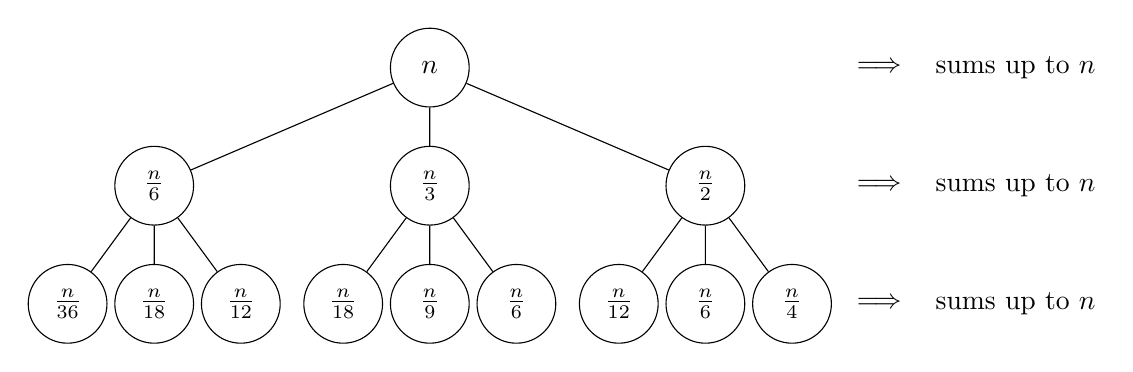
\begin{tikzpicture}[every node/.style={circle,draw,minimum size=1cm},level 1/.style={sibling distance=35mm},level 2/.style={sibling distance=11mm}]
			\node(Root){$n$}		
				child { node{$\frac n6$}
					child { node{$\frac n{36}$} }
					child { node{$\frac n{18}$} }
					child { node{$\frac n{12}$} }
				}
				child { node{$\frac n3$}
					child { node{$\frac n{18}$} }
					child { node{$\frac n9$} }
					child { node{$\frac n6$} }
				}
				child { node{$\frac n2$}
					child { node{$\frac n{12}$} }
					child { node{$\frac n6$} }
					child { node{$\frac n4$} }
				}
			;
			\begin{scope}[every node/.style={right}]
				\path (Root    -| Root-3-3) ++(7mm,0) node {$\Longrightarrow$} ++(10mm,0) node {sums up to $n$};
				\path (Root-1  -| Root-3-3) ++(7mm,0) node {$\Longrightarrow$} ++(10mm,0) node {sums up to $n$};
				\path (Root-1-1-| Root-3-3) ++(7mm,0) node {$\Longrightarrow$} ++(10mm,0) node {sums up to $n$};
			\end{scope}
		\end{tikzpicture}
	\end{figure}
	\noindent
	Може да забележим, че на всяко ниво сбора на нехомогенните части дава точно $n$. Освен това дървото е пълно до ниво $\lceil log_6(n)\rceil$\footnote{Може да докажем тези две твърдения с индукция и да докажем формално сумата от всички върхове, че е в интервала $[n\,log_6(n),n\,log_2(n)]$, откъдето да получим асимптотиката $\Theta(n\,log(n))$. В текущия курс няма да правим индукции от такъв характер.\label{footnote-recursion-tree}} (при база $n=1$), съответно дървото е с височина $\lceil log_2(n)\rceil$\hyperref[footnote-recursion-tree]{\footnotemark[\thefootnote]}. Тоест заподозряхме, че $T(n)=\Theta(n\,log_2(n))+O\big(n(log_6(n)-log_2(n))\big)=\Theta(n\,log(n))$. Сега ще го докажем формално. Нека $n_{st}\in\mathbb{N}_0$ е достатъчно голямо.
	\begin{itemize}
		\item $T(n)=O(n\,log(n))$
		
		По $\hyperref[bdef-asymp-classes]{\text{дефиниция}}$ $O(n\,log(n))\!=\!\{f\in\mathscr{F}^+|\big(\exists c\!>\!0\big)\big(\exists n_0\!\in\!\mathbb{N}_0\big)\big(\forall n\!\ge\! n_0\big)\big(0\!\le\! f(n)\!\le\! cn\,log(n)\big)\}$. Тоест търсим $c>0$ и $n_0\in\mathbb{N}_0$ такива, че $\big(\forall n\ge n_0\big)\big(T(n)\le n\,log(n)\big)$.
		
		Нека $b=\max\Bigl\{\frac{T(2)}{2log(2)},\frac{T(3)}{3log(3)},\dots,\frac{T(n_{\text{st}}-1)}{(n_{\text{st}}-1)log(n_{\text{st}}-1)},1\Bigr\}$. (виж $\remref{rem:rec-base}$)
		
		Ще докажем с индукция по $n$, че за $c=b$ и някое $n_0$ (което ще установим по-надолу) е изпълнено $\big(\forall n\ge n_0\big)\big(T(n)\le n\,log(n)\big)$.
		
		\begin{base}
			Нека $k\in\{2,3,\dots,n_{st}-1\}$. Ще докажем, че $T(k)\le b\,k\,log(k)$.
			
			От дефиницията на $b=\max\Bigl\{\frac{T(2)}{2log(2)},\frac{T(3)}{3log(3)},\dots,\frac{T(n_{\text{st}}-1)}{(n_{\text{st}}-1)log(n_{\text{st}}-1)},1\Bigr\}$ знаем, че $b\ge \frac{T(k)}{k\,log(k)}$ откъдето $b\,k\,log(k)\ge T(k)$ или още $T(k)\le b\,k\,log(k)$.
		\end{base}
		
		\begin{indhypothesis}
			Нека допуснем, че е изпълнено $\big(\forall m<n\big)\big(T(m)\le b\,m\,log(m)\big)$.
		\end{indhypothesis}
		
		\begin{indstep}
			Ще докажем, че е изпълнено за $n$, тоест че $T(n)\le bn\,log(n)$.
			\begin{equation*}
				T(n)\overset{\text{def}}{=}T\Big(\frac n6\Big)+T\Big(\frac n3\Big)+T\Big(\frac n2\Big)+n\overset{\text{ИХ}}{\le}\frac {bn}6log\Big(\frac n6\Big)+\frac {bn}3log\Big(\frac n3\Big)+\frac {bn}2log\Big(\frac n2\Big)+n\overset{?}{\le}bn\,log(n)
			\end{equation*}
			\begin{equation*}
				\frac{bn}6\big(log(n)-log(6)\big)+\frac{bn}3\big(log(n)-log(3)\big)+\frac{bn}2\big(log(n)-log(2)\big)+n\overset{?}{\le}bn\,log(n)
			\end{equation*}
			\begin{equation*}
				bn\,log(n)+\bigg(1-\frac{b\,log(6)}6-\frac{b\,log(3)}3-\frac{b\,log(2)}2\bigg)n\overset{?}{\le}bn\,log(n)
			\end{equation*}
			\begin{equation*}
				\bigg(1-\frac{b\,log(6)}6-\frac{b\,log(3)}3-\frac{b\,log(2)}2\bigg)n\overset{?}{\le}0
			\end{equation*}
			
			
			Може да забележим, че при $\frac{b\,log(6)}6+\frac{b\,log(3)}3+\frac{b\,log(2)}2\ge1$ горното неравенство ще е изпълнено за всяко $n\ge1$. Оттук си избираме $n_0=2$ (при $n_0=1$ имаме $\frac{T(1)}{1log(1)}=\frac{T(1)}0$).
			
			Остана да видим кога е изпълнено $\frac{b\,log(6)}6+\frac{b\,log(3)}3+\frac{b\,log(2)}2\ge1$. Очевидно е изпълнено когато $b\ge1$. Това сме си го подсигурили от дефиницията на $b=\max\{\dots,1\}\Rightarrow b\ge1$.
		\end{indstep}
		
		Тоест доказахме, че за $c=b$ и $n_0=1$ е изпълнено $\big(\forall n\ge n_0\big)\big(0\le T(n)\le cn\,log(n)\big)$. Казано с други думи $T(n)=O(n\,log(n))$.
		
		\vspace{0.35cm}
		\item $T(n)=\Omega(n\,log(n))$ - Докажете за упражнение.
	\end{itemize}
	
	
\end{solution}\vspace{0.25cm}


\subsection{Теорема на Akra-Bazzi}

Сега ще разгледаме метод, който е строго по-силен от Мастър теоремата, която е твърде ограничена - има една единствена поява вдясно. Теоремата на Akra-Bazzi позволява решаването на частен случай рекурентни уравнения с една или повече появи вдясно.%\vspace{-2cm}

\begin{boxtheorem}{Akra-Bazzi}{akra-bazzi}
	%Нека $T(n)=a_1T(b_1n)+\dots+a_kT(b_kn)+f(n)$ за $n>n_0$ и $\Theta(1)$ иначе, където
	Нека $T(n)=\!\begin{cases}
		\theta(1)                   &\!\!\!\!\!,1\le n\le n_0\\
		a_1T(b_1n)+\dots+a_kT(b_kn)+f(n) &\!\!\!\!\!,n>n_0
	\end{cases}$, където
	\begin{enumerate}[label=\textbf{\arabic*.}]
		\item $1\le n\in\mathbb{R}$
		\vspace{-0.24cm}
		\item $\big(\forall i\in\{1,\dots,k\}\big)\big(n_0\ge\frac1{b_i}\land n_0\ge\frac1{1-b_i}\big)$
		\vspace{-0.25cm}
		\item $\big(\forall i\in\{1,\dots,k\}\big)\big(a_i>0\big)$
		\vspace{-0.2cm}
		\item $\big(\forall i\in\{1,\dots,k\}\big)\big(b_i\in(0,1)\big)$
		\vspace{-0.2cm}
		\item $k\in\mathbb{N}^+$
		\vspace{-0.2cm}
		\item $f(n)$ е неотрицателна функция, удволетворяваща условието за полиномиално нарастване
		\vspace{-0.46cm}
		\item $p$ е уникално число, за което $\sum\limits_{i=1}^ka_ib_i^p=1$
	\end{enumerate}
	Тогава
	\begin{equation*}
		T(n)\asymp n^p\bigg(1+\displaystyle\int_1^n\frac{f(t)}{t^{p+1}}dt\bigg)
	\end{equation*}
\end{boxtheorem}

\hypersetup{linkcolor=green}
%\vspace{-1cm}
\begin{boxdefinition}{Условие за полиномиално нарастване (в$\,$контекста$\,$на $\thmref{th:akra-bazzi}$)}{poly-growth}
	Ще казваме, че $f(n)$ удволетворява условието за полиномиално нарастване, т.с.т.к. $\big(\exists c_1>0\big)\big(\exists c_2>0\big)\big(\forall n\ge1\big)\big(\forall i\in\{1,\dots,k\}\big)\big(\forall t\in[b_in,n]\big)\big(c_1f(n)\le f(t)\le c_2f(n)\big)$.
\end{boxdefinition}

\hypersetup{linkcolor=mydarkblue}

\begin{problem}
Каква е асимптотиката на $T(n)=\frac14T\big(\frac n4\big)+\frac34T\big(\frac{3n}4\big)+1$? 
\end{problem}

\begin{solution}
	Ще покажем, че седемте условия от $\hyperref[th:akra-bazzi]{\text{теоремата на Akra-Bazzi}}$ са изпълнени:
	\begin{enumerate}
		\item Това условие няма какво да го проверяваме.
		\vspace{-0.15cm}
		\item Проверяваме, че $n_0=4$ ни върши работа: $\big(\forall i\in\{1,2\}\big)\Big(4\ge\frac1{b_i}\land 4\ge\frac1{1-b_i}\Big)$.
		\vspace{-0.15cm}
		\item Директно проверяваме $\big(\forall i\in\{1,2\}\big)\big(a_i>0\big)$.
		\item Директно проверяваме $\big(\forall i\in\{1,2\}\big)\big(b_i\in(0,1)\big)$.
		\item Това условие няма какво да го проверяваме.
		\item Проверяваме, че $c_1\!=\!c_2\!=\!1$ са свидетели: $\big(\forall n\!\ge\!1\big)\big(\forall i\!\in\!\{1,2\}\big)\big(\forall t\!\in\![b_in,n]\big)\big(1\!\le\!1\!\le\!1\big)$.
		\item Проверяваме, че $p=0$ ни върши работа: $\frac14\big(\frac14\big)^0+\frac34\big(\frac34\big)^0=1$.
	\end{enumerate}
	\vspace{-0.2cm}
	Тогава прилагаме теоремата на Akra-Bazzi и получаваме $T(n)\asymp n^0\bigg(1+\displaystyle\int_1^n\frac1tdt\bigg)=\Theta(log(n))$.
\end{solution}\leavevmode\newline


\subsection{Задачи}

Основната идея за строене на рекурентно уравнение за сложността на рекурсивен алгоритъм е за всяко рекурсивно извикване с параметър $k$ да добавим отдясно на равенството $T(k)$. Останалата \emph{работа} ще представлява нехомогенната част на рекурентното уравнение.\\

\begin{problem}
	Даден е следният алгоритъм:
	\begin{pseudocode}
		\SetKwData{di}{i}
		\SetKwData{dn}{n}
		\SetKwData{dnn}{n\,-\,1}
		\SetKwData{ds}{s}
		
		
		$Func(\dn)://\,\dn\in\mathbb{N}^+$
		\Mybegin
		{
			$\ds\leftarrow0$\;
			\Myfor{$\di\leftarrow1$ \KwTo $\dnn$}{$\ds\leftarrow\ds+2*Func(\di)+1$\;}
			\KwRet{$\ds$}\;
		}
	\end{pseudocode}
	Каква е сложността му по време (спрямо $n$)?
\end{problem}

\begin{solution}
	Имаме $n-1$ на брой рекурсивни извиквания.. това означава, че за всяко едно от тях трябва да добавим отдясно на равенството $T(\text{\emph{подходящ параметър}})$. Останалата \emph{работа} в случая е инициализацията на $s$, инкрементацията на $i$ и актуализацията на $s$, т.е. $\Theta(n)$. Тя може да се погълне от рекурсивните извиквания (по единица на извикване). Тоест рекурентното уравнение е $T(n)=T(n-1)+T(n-2)+\dots+T(1)+\Theta(1)$. Вече намерихме асимптотиката на подобно рекурентно уравнение в $\probref{prob-rec-eq-full-history}$.
	\begin{center}
		$\begin{array}{|l}
			T(n)=T(n-1)+T(n-2)+\dots+T(1)+\Theta(1)\\
			T(n-1)=T(n-2)+T(n-3)+\dots+T(1)+\Theta(1)
		\end{array}$
	\end{center}
	Тогава $T(n)-T(n-1)=T(n-1)+\Theta(1)-\Theta(1)$ или още $T(n)=2T(n-1)+\Theta(1)$. Вече може да го решим чрез метода с характеристично уравнение.
	\begin{itemize}
		\item (Хомогенна част)\\
		$x=2\ \mapsto\ \{2\}_M$
		
		\item (Нехомогенна част)\\
		$\Theta(1)\ \mapsto\ \{1\}_M$
	\end{itemize}
	Оттук получаваме, че $T(n)=c_11^n+c_22^n=\Theta(2^n)$.
\end{solution}\leavevmode\newline

\begin{problem}
	Даден е следният алгоритъм:
	\begin{pseudocode}
		\SetKwData{di}{i}
		\SetKwData{dn}{n}
		\SetKwData{dnn}{n\,-\,1}
		\SetKwData{ds}{s}
		
		
		$Func(\dn)://\,\dn\in\mathbb{N}^+$
		\Mybegin
		{
			$\ds\leftarrow0$\;
			\Myfor{$\di\leftarrow1$ \KwTo $\dnn$}{$\ds\leftarrow\ds+Func(\di)+Func(\di)+1$\;}
			\KwRet{$\ds$}\;
		}
	\end{pseudocode}
	Каква е сложността му по време (спрямо $n$)?
\end{problem}

\begin{solution}
	Имаме $2(n-1)$ на брой рекурсивни извиквания.. това означава, че за всяко едно от тях трябва да добавим отдясно на равенството $T(\text{\emph{подходящ параметър}})$. Останалата \emph{работа} в случая е инициализацията на $s$, инкрементацията на $i$ и актуализацията на $s$, т.е. $\Theta(n)$, което отново може да се погълне от рекурсивните извиквания. Тоест рекурентното уравнение е $T(n)=2T(n-1)+2T(n-2)+\dots+2T(1)+\Theta(1)$.
	\begin{center}
		$\begin{array}{|l}
			T(n)=2T(n-1)+2T(n-2)+\dots+2T(1)+\Theta(1)\\
			T(n-1)=2T(n-2)+2T(n-3)+\dots+2T(1)+\Theta(1)
		\end{array}$
	\end{center}
	Тогава $T(n)-T(n-1)=2T(n-1)+\Theta(1)-\Theta(1)$ или още $T(n)=3T(n-1)+\Theta(1)$. Вече може да го решим чрез метода с характеристично уравнение.
	\begin{itemize}
		\item (Хомогенна част)\\
		$x=3\ \mapsto\ \{3\}_M$
		
		\item (Нехомогенна част)\\
		$\Theta(1)\ \mapsto\ \{1\}_M$
	\end{itemize}
	Оттук получаваме, че $T(n)=c_11^n+c_23^n=\Theta(3^n)$.
\end{solution}